 
\documentclass[12pt]{article}
\usepackage{graphicx}
\usepackage{caption}
\usepackage{subcaption}
\usepackage{amsmath}
\usepackage{hyperref}

\title{Machine Learning for Object Detection and Classification of Defects on Printed Circuit Boards (PCBs)}
\author{Faiza Waheed, Niels Hartano and Gernot Gellwitz}
\date{\today}

\begin{document}

\maketitle

\begin{abstract}
This report presents a machine learning approach for detecting and classifying defects on printed circuit boards (PCBs). The aim is to enhance the quality control process in PCB manufacturing by leveraging advanced computer vision techniques.
\end{abstract}

\section{Introduction}
Printed Circuit Boards (PCBs) are essential components in nearly all electronic devices. Ensuring their quality is critical, as defects can lead to device malfunctions or failures. Traditional inspection methods, often manual, are time-consuming and prone to human error. 

Machine learning, particularly deep learning, has shown significant promise in automating and improving the accuracy of defect detection and classification in PCBs. By training models on annotated images of PCBs, these systems can learn to identify various types of defects such as solder joint issues, component misalignments, and surface contamination.

This project focuses and compares two approaches for defect detection and classificaion: The first approach is based on the vgg16 network, the second is 
based on U-Net. The former makes use of so-called bounding boxes to detect defects, while the latter uses segmentation to classify defects.
Vgg16 can be downloaded as a pretrained model on from the tensorflow-keras library, while U-Net has to be implemented from scratch. Vgg16 therefore can be utilized for transfer learning.

\begin{figure}[h]
    \centering
    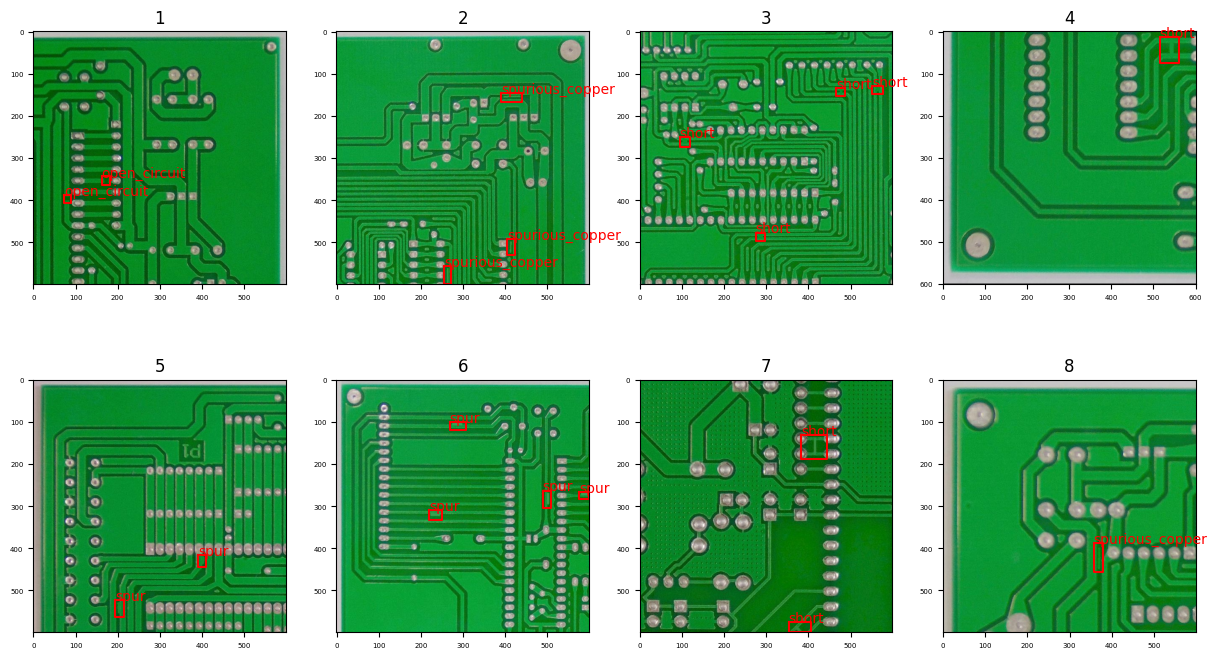
\includegraphics[width=0.8\textwidth]{./graphics/4.png}
    \caption{Sample images from the PCB dataset with annotated defects.}
\end{figure}

We were given a large dataset of around 10.000 PCB images with a total of arround 22.000 annotated defects, which we used to train and evaluate our models. The goal was to develop a robust system capable of detecting and classifying defects with high accuracy and efficiency.
The dataset can be downloaded from kaggle: \url{https://www.kaggle.com/datasets/akhatova/pcb-defects }

\begin{figure}[h]
    \centering
    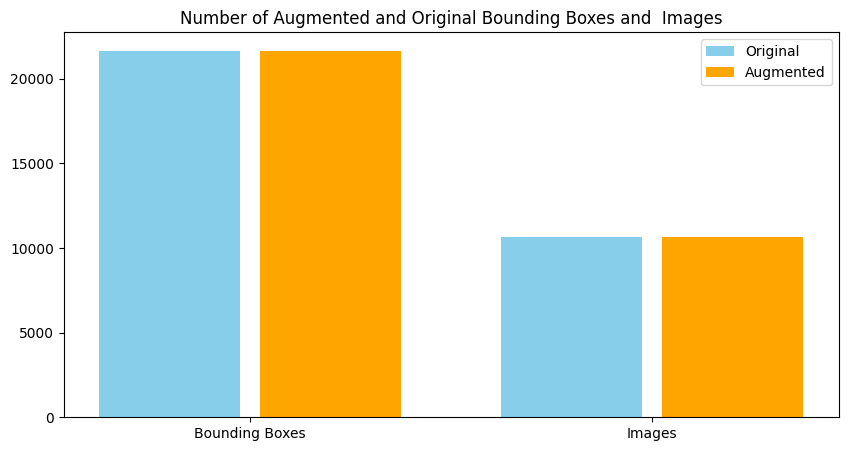
\includegraphics[width=0.8\textwidth]{./graphics/2.png}
    \caption{Ratio of Number of defects to Number of images}
\end{figure}

Some images only contained one defect, while others contained multiple defects. (See Fig. 1.)

Over all 6 different classes of defects were considered:
\begin{itemize}
    \item Mouse Bites
    \item Missing Components
    \item Short
    \item Spurious Copper
    \item Missing Holes
    \item Open Circuits
\end{itemize}

These defects were fairly distributed in the dataset, with the most common defect being "Mouse Bites" and the least common defect being "Shorts".

\begin{figure}[h]
    \centering
    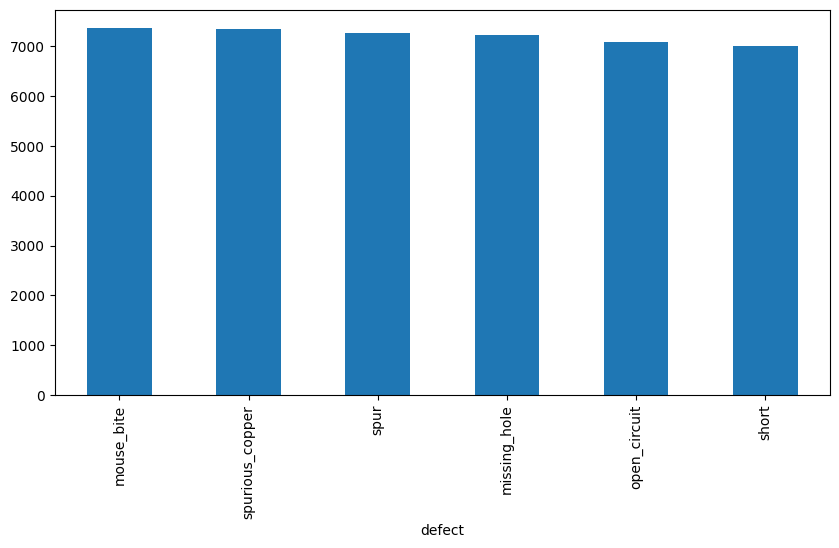
\includegraphics[width=0.8\textwidth]{./graphics/1.png}
    \caption{Defect distribution.}
\end{figure}

The main objectives were to:
\begin{itemize}
    \item Create a datafram from around 10.000 ".xml" annotation files in an ".xml" format containing the dimensions of the bounding boxes, size of the pictures and the type of defect.
    \item Preprocess the data by creating augmentations.
    \item Train a model to detect and classify defects.
    \item Evaluate the model's performance and optimize it for deployment in a production environment.
\end{itemize}

\subsection{Preprocessing}
A high-quality dataset is crucial for training an effective model. Data augmentation is a crucial technique in machine learning, 
particularly for tasks involving image data, such as object detection and classification of defects on printed circuit boards (PCBs). 
By artificially expanding the training dataset through transformations like rotations, flips, scaling, and translations, data augmentation 
helps improve the robustness and generalization ability of the model. This process mitigates overfitting by exposing the model to a diverse 
set of variations and scenarios that it might encounter in real-world applications. Consequently, data augmentation enhances the model's 
ability to accurately detect and classify defects, even when faced with new or slightly altered images, thereby improving its overall 
performance and reliability in practical deployment.

Two approaches were considered for data augmentation: Using a library or implementing the augmentations by hand. The former is more convenient and less error-prone, while the latter offers more flexibility and control over the augmentation process. 

\subsubsection{Augmentations via Albumentations}

The libary-based approach made use of the library "Albumentations", specifically techniques availlable where rondom brightness or contrast, random cropping of the image,
rotation, horizontal or vertical fippping, including random sun flares or changing of the hue saturation value. (See Fig. 4.)

\begin{figure}[h]
    \centering
    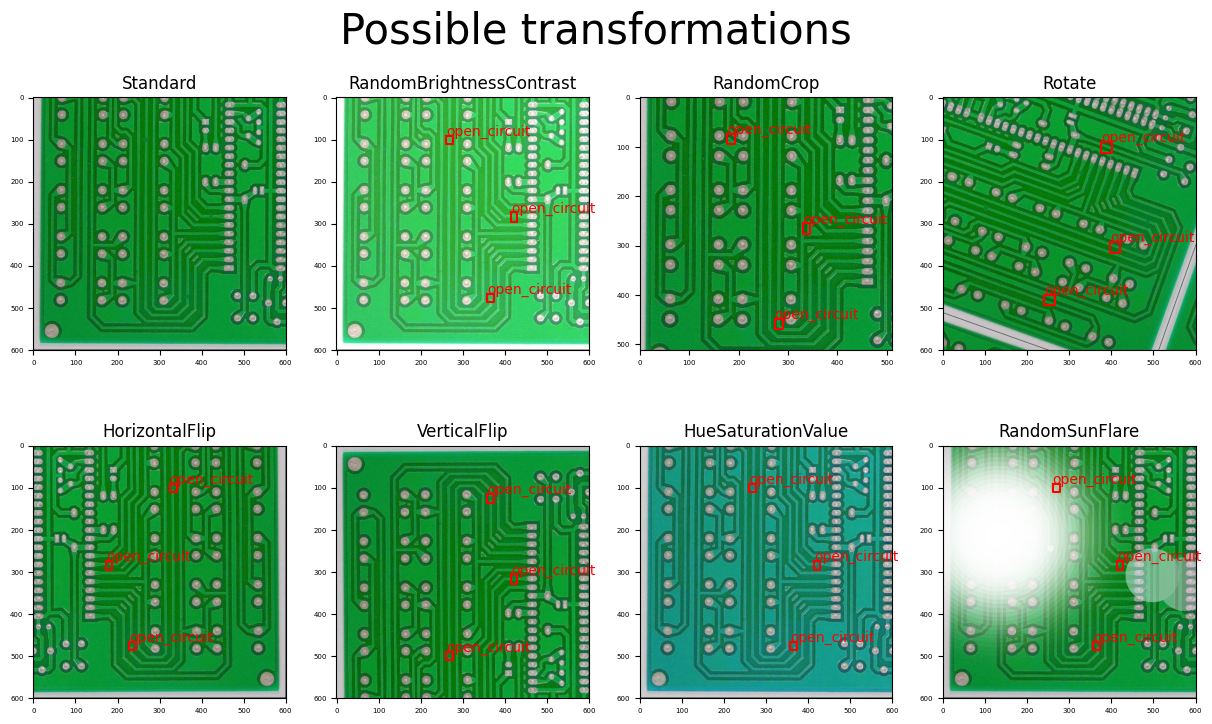
\includegraphics[width=0.8\textwidth]{./graphics/5.png}
    \caption{Possible augmentations by "Albumentations".}
\end{figure}

Problems that occured during this process were that the cropping of the images may lead to the loss of the defect, if the defect is located outside of the cropped part of the image, which is not desired.
In this case the defect would not be detected by the model. Another problem was that in the case of ratotion the defects were not correclty placed as can be seen in Fig. 4. That is why
cropping and rotation were not used in the final model.

\subsubsection{Augmentations by Hand}

...

\section{Modelling}
The methodology of this project involves several key steps: data frame generation and preprocessing, model design and training, and evaluation.


\subsection{Model Design and Training}

\subsubsection{Vgg16}

The VGG16 model is a convolutional neural network architecture that has been widely used for image classification tasks. It consists of 16 layers, including 13 convolutional layers and 3 fully connected layers. The model has been pre-trained on the ImageNet dataset, which contains millions of images across thousands of classes. By leveraging transfer learning, we can take advantage of the features learned by the model on ImageNet and fine-tune it on our PCB dataset.
The model was implemented using the TensorFlow and Keras libraries. 

VGG16 requires the following additional preprocessing steps: 

\begin{itemize}
    \item Resizing images to a 224 by 224 image size to fit the model input requirements. All colors where kept
    \item Normalizing pixel values to the range [0, 1].  
\end{itemize}

Furthermore the dimensions of the bounding box where normalized and centered. The defects had to be split up by using a One-Hot-Encoding. The dataset was then split into a training and a validation set. 
TensorFlow additionally requires the transformation of the dataset into a tf.data.Dataset object.

Two appreoches were tested: freezing (keeping) all pretrained layers and only adding a flatten layer and an detection and an classification head and unfreezing all layers.

\begin{figure}[h]
    \centering
    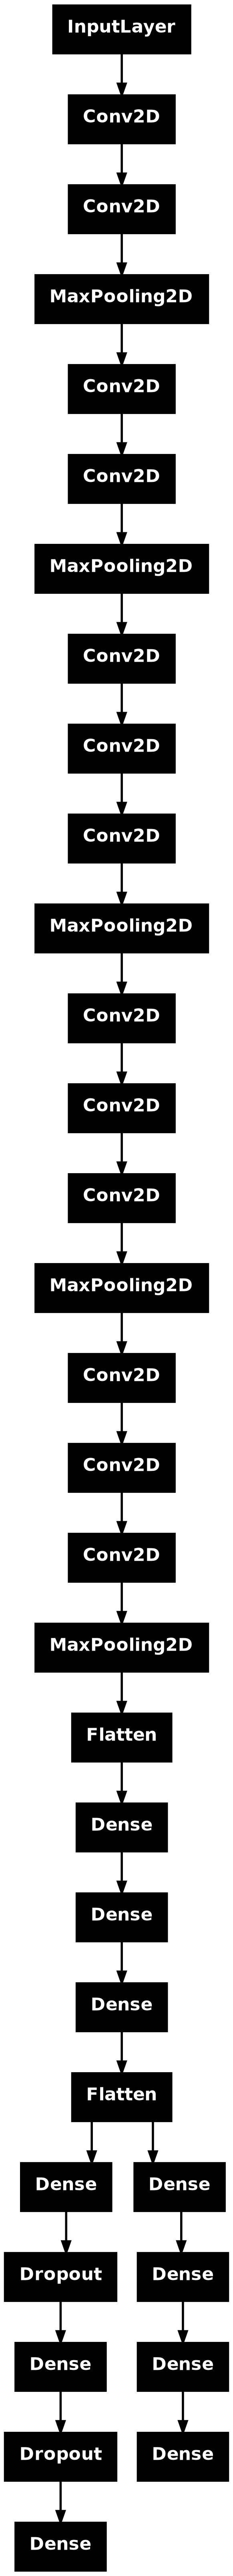
\includegraphics[width=0.14\textwidth]{./graphics/3.png}
    \caption{Vgg16 with two heads.}
\end{figure}

Using two different heads enables the user to use differenct loss functions and metrics for the detection and classification task. 
For the detection task the loss function GIoU and metrics One-Hot-IOU was used, while for the classification task the loss function categorical crossentropy and metrics accuracy were used.

To avoid unnecessary computation, callbacks were implemented such as early stopping and model checkpointing. 


\subsubsection{U-Net}

...


\subsection{Evaluation}

...


\section{Conclusion}

\end{document}